\section{Hiện thực trò chơi}
\subsection{UI trong màn chơi}
Phần lớn các UI trong trò chơi đều được kế thừa từ class CanvasBaseView nhằm tái sử dụng những chức năng cơ bản như: hiện, ẩn hoặc toggle giữa 2 trạng thái.
\begin{figure}[H]
	\centering
	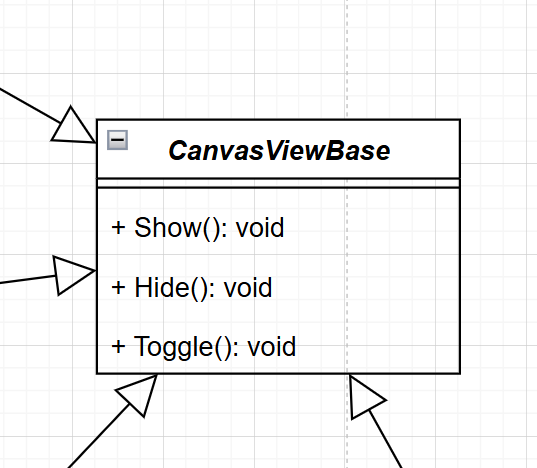
\includegraphics[width=7cm]{Images/CanvasViewBase.png}
	\vspace{0.5cm}
	\caption{CanvasViewBase}
\end{figure}

\subsubsection{UI tham khảo schema diagram}
\begin{figure}[H]
	\centering
	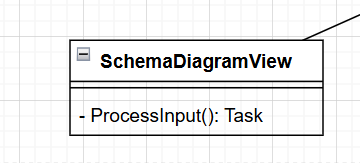
\includegraphics[width=7cm]{Images/SchemaDiagramView.png}
	\vspace{0.5cm}
	\caption{Schema diagram view}
\end{figure}

\begin{figure}[H]
	\centering
	\includegraphics[width=13cm]{Images/SchemaDiagramUi.png}
	\vspace{0.5cm}
	\caption{Minh họa UI Schema diagram view}
\end{figure}

\subsubsection{UI cấu trúc màn chơi}
\begin{figure}[H]
	\centering
	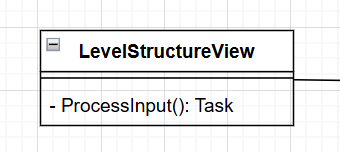
\includegraphics[width=7cm]{Images/LevelStructureView.png}
	\vspace{0.5cm}
	\caption{Level structure view}
\end{figure}

\begin{figure}[H]
	\centering
	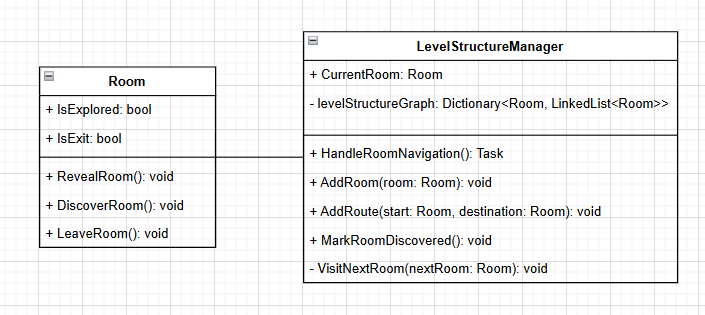
\includegraphics[width=13cm]{Images/LevelStructureManager.png}
	\vspace{0.5cm}
	\caption{Level structure manager}
\end{figure}

\begin{figure}[H]
	\centering
	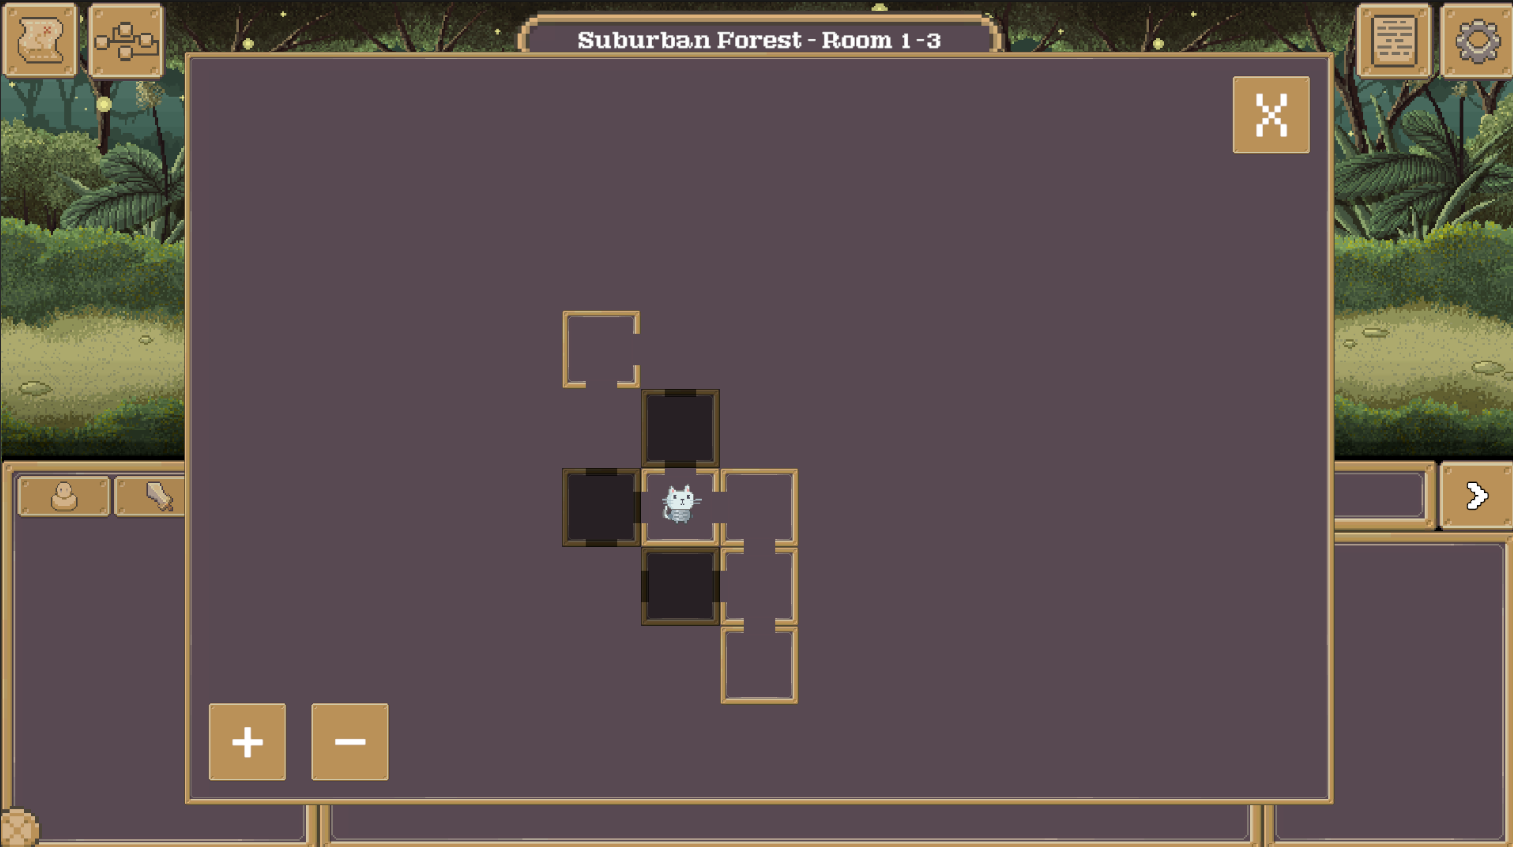
\includegraphics[width=13cm]{Images/LevelStructureUI.png}
	\vspace{0.5cm}
	\caption{Minh họa UI cấu trúc màn chơi}
\end{figure}

\subsubsection{UI tham khảo cú pháp SQL cơ bản}
\begin{figure}[H]
	\centering
	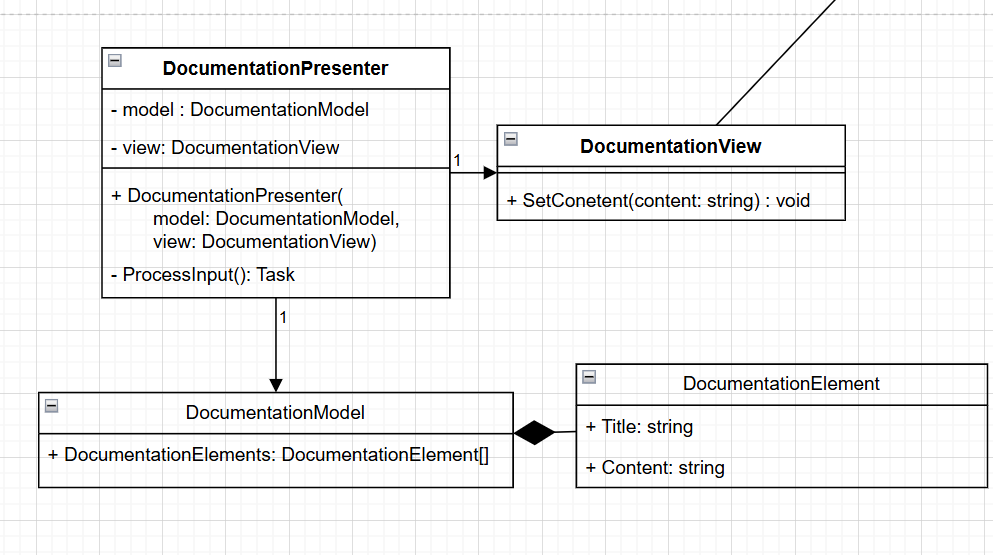
\includegraphics[width=13cm]{Images/DocumentationView.png}
	\vspace{0.5cm}
	\caption{Documentation class diagram}
\end{figure}

\begin{figure}[H]
	\centering
	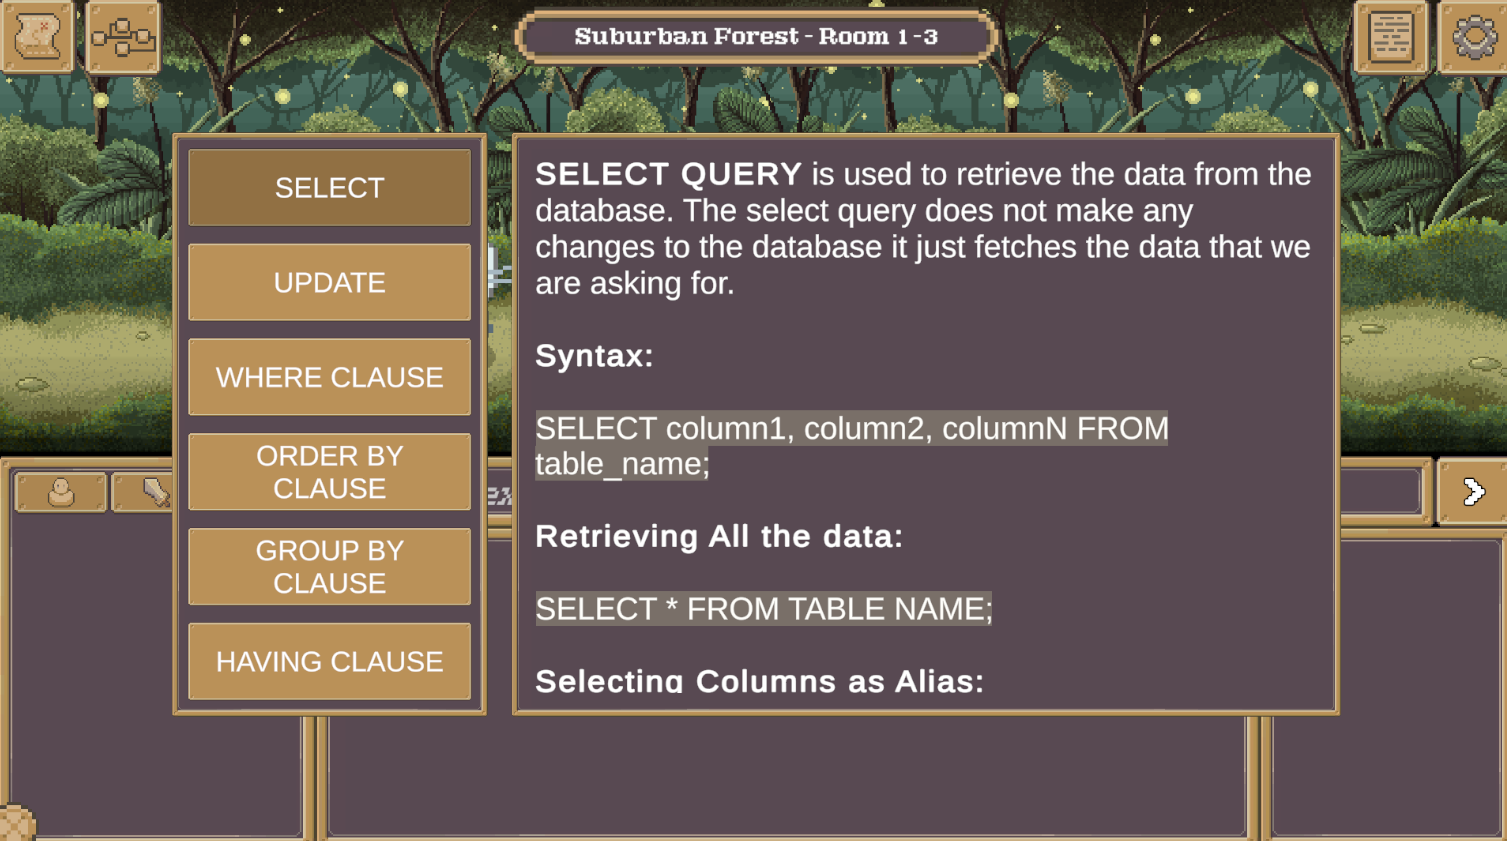
\includegraphics[width=13cm]{Images/DocumentationUI.png}
	\vspace{0.5cm}
	\caption{Minh họa UI tra cứu câu lệnh SQL}
\end{figure}

\subsubsection{Hội hội thoại}
\begin{figure}[H]
	\centering
	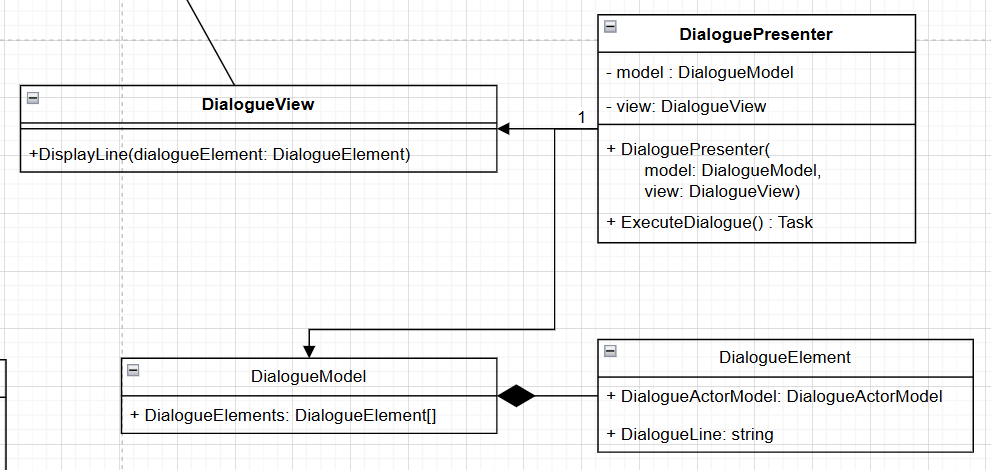
\includegraphics[width=13cm]{Images/DialogueView.png}
	\vspace{0.5cm}
	\caption{Dialogue class diagram}
\end{figure}

\begin{figure}[H]
	\centering
	\includegraphics[width=13cm]{Images/DialogueUI.png}
	\vspace{0.5cm}
	\caption{Minh họa UI đoạn hội thoại}
\end{figure}

\subsubsection{Hiệu ứng pop up text}
\begin{figure}[H]
	\centering
	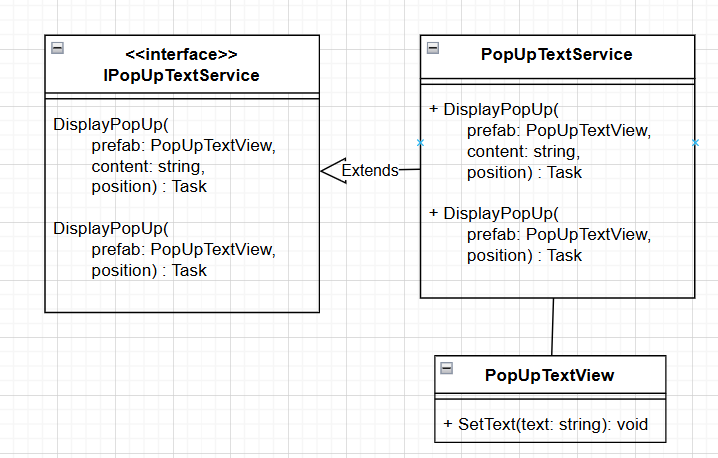
\includegraphics[width=13cm]{Images/PopUpText.png}
	\vspace{0.5cm}
	\caption{Pop up text class diagram}
\end{figure}

\begin{figure}[H]
	\centering
	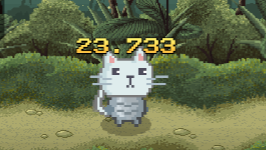
\includegraphics[width=13cm]{Images/PopupTextUI.png}
	\vspace{0.5cm}
	\caption{Minh họa UI Popup text}
\end{figure}

\subsubsection{Hộp thoại thông báo}
\begin{figure}[H]
	\centering
	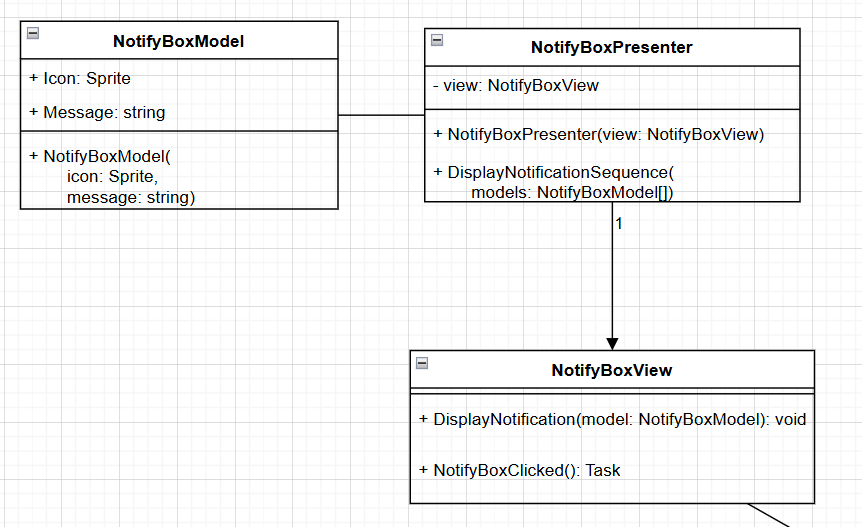
\includegraphics[width=13cm]{Images/NotifyBoxView.png}
	\vspace{0.5cm}
	\caption{Notify box class diagram}
\end{figure}

\begin{figure}[H]
	\centering
	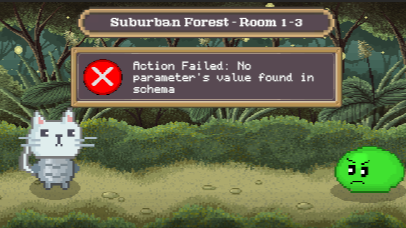
\includegraphics[width=13cm]{Images/NotifyBoxUI.png}
	\vspace{0.5cm}
	\caption{Minh họa UI hộp thoại thông báo}
\end{figure}